\chapter{Nested association mapping analysis for chickpea hybrids}
\label{cha:research_topic_2}

\section{Introduction}

Cultivated chickpea (\textit{C. arietinum}), a small herbaceous plant, is the world's second most important pulse legume and is one of the earliest cultivated legumes \cite{vonWettberg2018, Sani2018}, with particular importance in the semi-arid tropics of sub-Saharan Africa and South Asia. Domesticated chickpea is believed to have diverged from its closest wild relative \textit{C. reticulatum} (fig. \ref{fig:cicer-phylo}) around 10,000 years ago \cite{vonWettberg2018}. 

\begin{figure}[h!]
    \centering
    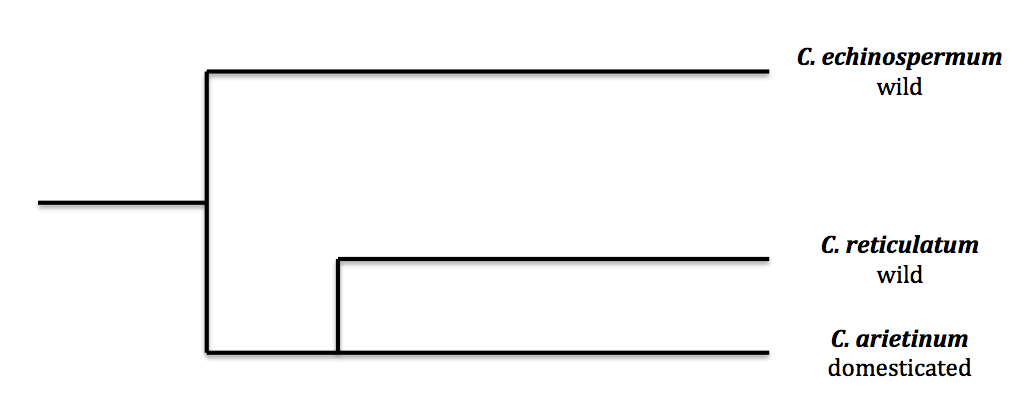
\includegraphics[scale=0.8]{tex/chickpea/chickpea.png}
    \caption{Phylogenetic relationships in chickpea (\textit{cicer}).}
    \label{fig:cicer-phylo}
\end{figure}


The process of domestication and breeding has unintended consequences for a species. The nature and 
intensity of artificial selection imposed by breeders can impart genetic drift, reduce diversity and increase the frequency of deleterious alleles. This reduced diversity and fixation of deleterious alleles has varied implications - it constrains our ability to expand the cultivation of crops into environments that differ from those under which domestication occurred and the reduced diversity makes the crop susceptible to  changing climate and pathogens. Indeed, in the case of the cultivated banana which is clonally propagated with extremely low diversity, the entire crop variety, \emph{Gros Michel}, has been wiped out by the Panama disease \cite{Ordonez2015}. A second wave of the Panama disease, similarly, threatens to wipe out the present \emph{Cavendish} banana variety \cite{Ordonez2015}. 

Domesticated chickpea has undergone an extreme domestication-related genetic bottleneck \cite{vonWettberg2018}. This has consequences for breeding of climate-resilient crop varieties, because much of the historical phenotypic plasticity necessary to tolerate environmental extremes may have been lost through domestication. Breeding only within cultivated material will have steeply diminishing returns, and there is an urgent need for new sources of diversity, for example, from wild material \cite{McCouch2013, Dempewolf2014, Hajjar2007}.

Sampling wild populations to make a genetic resource for the breeding community requires a consortium level effort. Keeping this goal in mind, the `Feed the Future Innovation Lab for Chickpea' was formed and has the objective of comprehensively characterizing a collection of wild species focused on \emph{C. reticulatum}, the wild progenitor of cultivated chickpea. Concurrently, we wish to develop a predictive network of genotype-phenotype associations that identifies genes and genome regions from wild species that improve chickpea's yield resilience to climatic extremes and helps bring back some of the lost diversity in to cultivated chickpea. 

Such programs have been carried out with great success in maize \cite{McMullen2009}, soybean \cite{Bandillo2017} and various other crops. Traditionally, linkage analysis, where crosses (back-cross or inter-cross generation) between two parents are made, has been used for the identification of genomic regions of interest affecting a particular phenotype. This approach relies on recent recombination and generally suffers from low resolution as the linkage blocks tend to be very large. Additionally, as we sample alleles from only two parents, there is low allelic richness in such mapping populations. A competing approach would be to sample populations from natural populations and rely on ancestral recombination. This approach has much better resolution but suffers from statistical power as the causative allele might be at low frequency in the population, requiring a large sample size to detect it. To alleviate concerns in both these approaches while still retaining the advantages of both, it was suggested to make a nested association mapping (NAM) \cite{McMullen2009} population for association mapping. 

In NAM populations, several founders (wild individuals) are crossed individually with a common cultivated parent. The F1 progeny are then selfed for a number of generations to produce recombinant inbred lines. %(fig. \ref{fig:nams}) 
NAM take advantage of both historic and recent recombination events and have advantages of low marker density requirements, high allele richness, high mapping resolution, and high statistical power \cite{Yu2008, McMullen2009}. 

%\begin{figure}
%    \centering
%    \includegraphics{}
%    \caption{Process of creating NAM populations}
%    \label{fig:nams}
%\end{figure}

In this chapter, we describe the NAM population developed for identifying genetic basis of agronomic traits in chickpea. A summary of the phenotypic distributions seen in the hybrids is also provided. We then assess how much of the variation can be attributed to additive and dominant effects. Lastly, we use a linear model to map the phenotypes onto genotypic data. 

\section{Materials and methods}

\subsection{Genotype and phenotype data}

19 diverse chickpea lines were chosen as the parental lines (fig. \ref{fig:wild-parent}) for the NAM population in order to encompass the remarkable diversity of chickpea and preserve historic linkage disequilibrium. Each parental line was crossed to the cultivar ICCV96029 (chosen as a reference line due to its wide deployment as one of the most successful commercial lines) to create the F1 population. The F1 plants were then self-fertilized for one generation in order to create a total of around 100 F2s per family, for a total of 2139 F2s within the NAM population (fig. \ref{fig:crosses}).

Each cross was then sequenced using genotype-by-sequencing \cite{He2014} techonology. Genotyping-by-sequencing offers a rapid and cost-effective means to identify genome-wide nucleotide variation in crop germplasm. The NAM lines were sequenced to a coverage of around 5X and aligend to the 2013 chickpea reference \cite{Varshney2013}. The shallow coverage led to an over-representation of homozygous calls. TASSEL's FSFHap algorithm \cite{Swarts2014}, was used to correct variant calls in the sequenced lines. To assess problems with the called genotypes, one of the cross families (ICCV96029 x Besev\textunderscore079) was analysed for recombination events. Fig. \ref{fig:unimputed-res} shows the number of recombination events (REs) per site as assessed by a change in phase (from homozygous wild, homozygous cultivated or heterozygous to another state) along the genome. As we can see, for a family size of 80 individuals, almost half the indidividuals show an RE. This is contrary to what is expected. Fig. \ref{fig:imputed-res} shows a similar plot but after imputation. As we can see, the number of REs per site has gone down significantly. There remain peaks where the REs per site are very high. We think that these regions reflect problems with the 2013 draft and are essentially misassembled regions that the imputation algorithm cannot fix. 

\begin{figure}
    \centering
    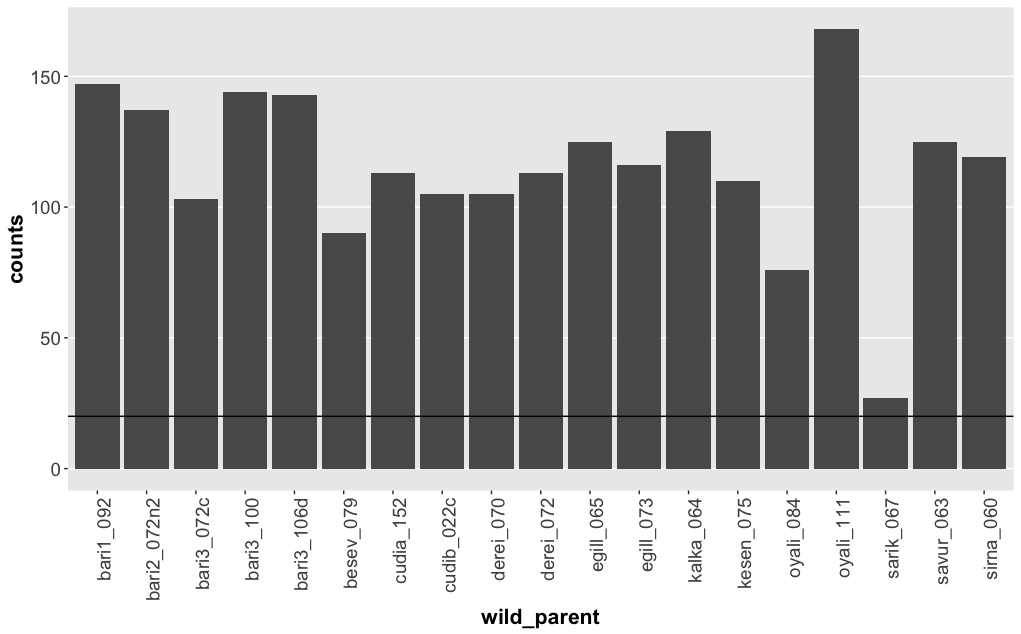
\includegraphics[scale = 0.4]{tex/chickpea/wild_parent.jpeg}
    \caption{Chickpea wild parents sampled from diverse regions in Turkey. X-axis shows the name of each founder and Y-axis represents the number of times the line participated in a cross.}
    \label{fig:wild-parent}
\end{figure}

\begin{figure}
    \centering
    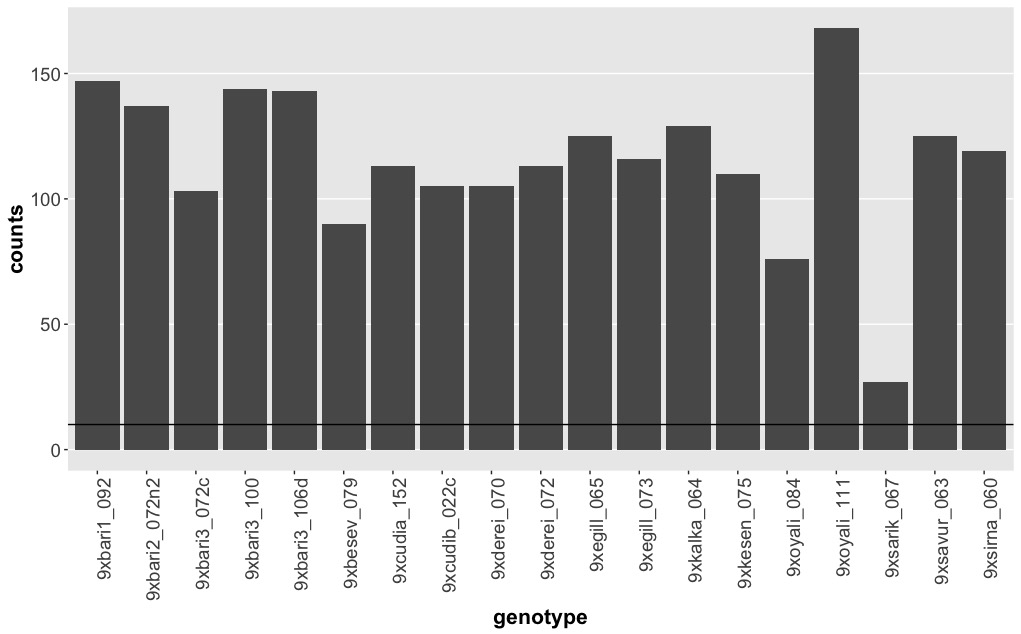
\includegraphics[scale=0.4]{tex/chickpea/crosses.jpeg}
    \caption{NAM crosses. X-axis represents the cross name and y-axis is the number of individuals in a particular family.}
    \label{fig:crosses}
\end{figure}

\begin{figure}
    \centering
    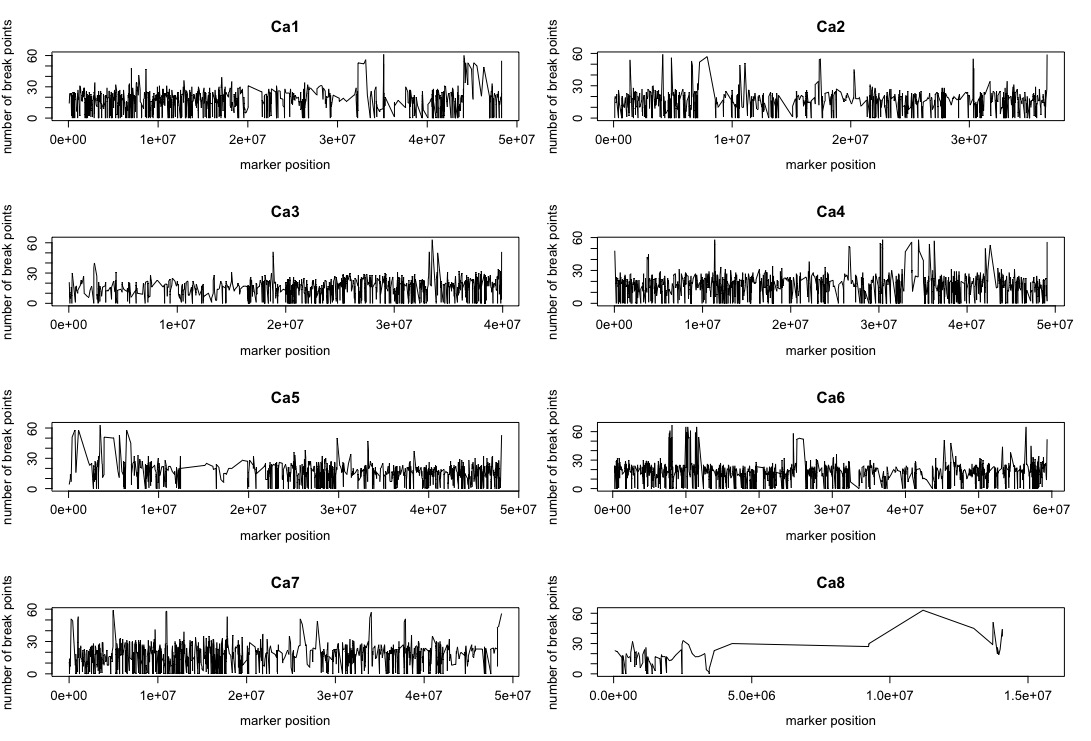
\includegraphics[height = 15cm, width = 15cm]{tex/chickpea/unimputed-res.jpeg}
    \caption{Recombination events along the chromosome for unimputed data for the ICCV96029 and Besev\textunderscore079 cross. Nearly half the individuals show a recombination each position, indicating that the gentoypic data is very noisy. The expected number of recombinations is extremely low as we deal with an F2 cross. X-axis: marker position (in bps). Y-axis: number of break points.}
    \label{fig:unimputed-res}
\end{figure}

\begin{figure}
    \centering
    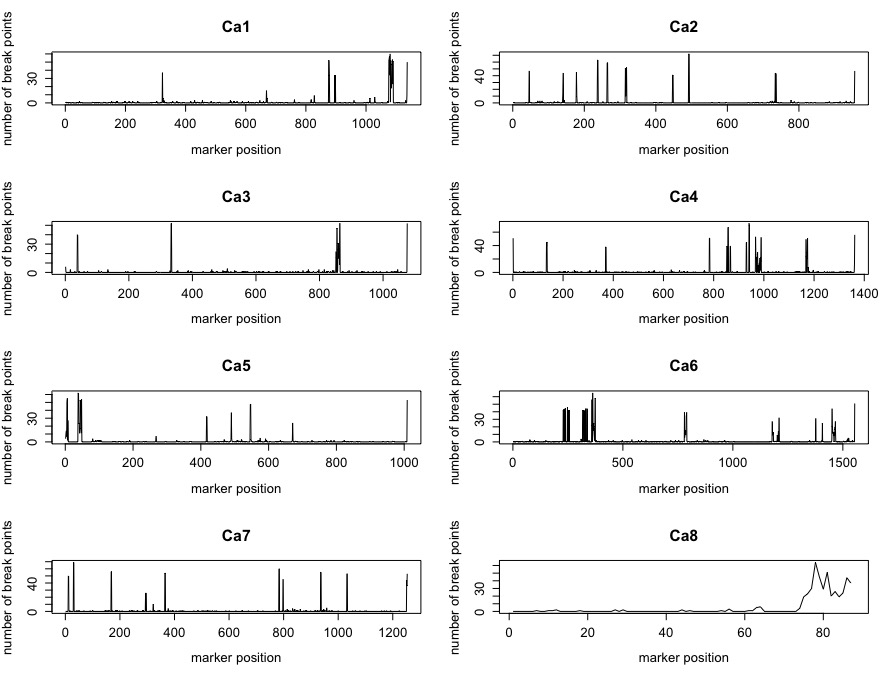
\includegraphics[height = 15cm, width = 15cm]{tex/chickpea/imputed-res.jpeg}
    \caption{Similar to fig. \ref{fig:unimputed-res} but now plotted with imputed data. The number of REs has dropped significantly except for certain regions. These regions could not be corrected by the algorithm and were particularly noisy. We believe they might represent problematic regions with the reference draft.}
    \label{fig:imputed-res}
\end{figure}

The F2s were grown using a common garden design and several phenotypes were collected. We selected 6 agronomically relevant phenotypes for this study that are listed below:

\begin{enumerate}
    \item \textbf{Total plant biomass}: total mass of the plant
    \item \textbf{Plant volume}: total volume of the plant; measured by immersing plant in water
    \item \textbf{Average mass of seed}: total mass of seeds divided by the total number of seeds
    \item \textbf{Yield}: total mass of seeds
    \item \textbf{Harvest index}: total mass of seeds as a percentage of the total above ground mass of plant
    \item \textbf{Shattering index}: total number of seeds that are shattered (dispersed) as a percentage of the total number of seeds
\end{enumerate}

\subsection{Marker selection}

The markers selection was done based on two criteria.
\begin{enumerate}
    \item For the segregation distortion analysis, the variants were filtered for 1\% minor allele frequency
    \item For the association mapping analysis, the markers were first separately filtered for intermediate frequency (35\%) by family. The markers were then imputed to correct for erroneous calls and then all the markers across families were combined together. The combined set was filtered for a missingness rate of 20\%. The combined set was then used for association mapping. 
\end{enumerate}
Fig. \ref{fig:marker-by-length} shows the number of markers versus the length of the chromosome. We see that chromosome 8, the smallest chromosome, has the least number of markers. Besides the length, chromosome 8 also suffers from distortion, thus, most of the markers do not meet the intermediate frequency requirement. 

\begin{figure}
    \centering
    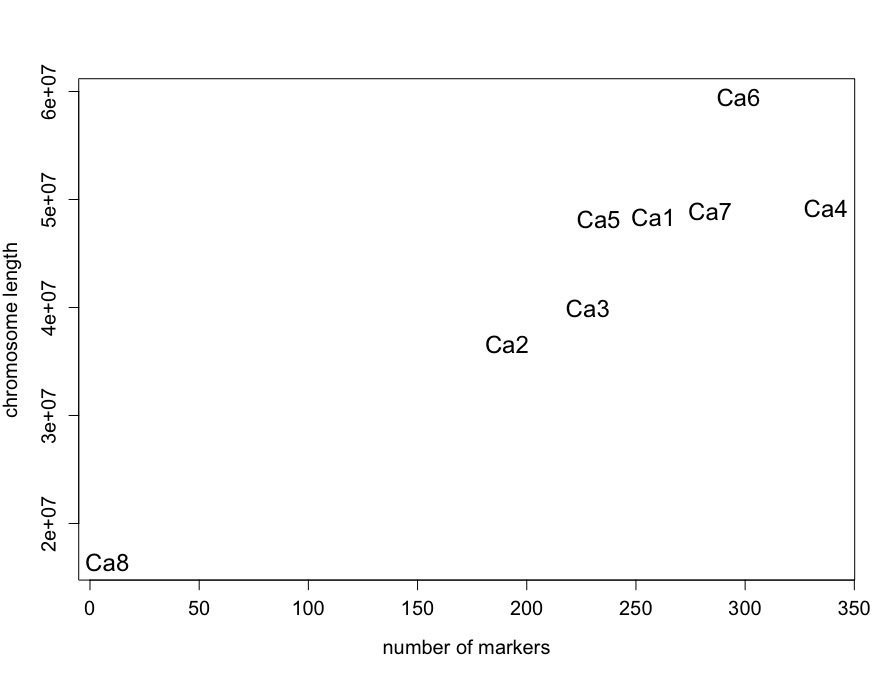
\includegraphics[scale = 0.45]{tex/chickpea/marker-by-length.jpeg}
    \caption{Number of markers (x-axis) used for association mapping analysis versus the length of the chromosome (y-axis) }
    \label{fig:marker-by-length}
\end{figure}

\subsection{Mixed models and heritability estimates}

Linear mixed models (LMMs) describe the outcome variable $Y$ as a linear combination of deterministic (fixed) effects and random effects. Random effect is the realization of a random variable whose distribution we try to model:

$$Y = \underbrace{X\beta}_{fixed\ effects} + \underbrace{Zb}_{random\ effects} + \underbrace{\epsilon}_{noise}.$$

LMMs can be used for heritability estimation in genetic analysis of plant and animal breeding \cite{Ogunniyan2014,Valdar2006}. We can consider all the markers for together as random effects in a genotypic model:

$$Y = X\beta + \sum_{i=1}^{m}W_ia_i + \sum_{i=1}^{m}Z_id_i + \epsilon,$$
where $Y$ is the outcome variable, $X$ is the design matrix for co-variates, $W_i$ accounts for the additive allele coding of the wild allele and $Z_i$ accounts for the dominance allele coding, $\epsilon$ is the unmodeled noise. The coefficients $\beta$, $a_i$ and $d_i$, account for the co-variate (fixed), additive (random effects) and dominance (random effects) deviation respectively. We assume that $a_i \sim N(0, \frac{\sigma^2_a}{m})$ and $d_i \sim N(0, \frac{\sigma^2_d}{m})$ where $\sigma_a^2$ and $\sigma_d^2$ is the additive and dominance variation explained jointly by all, $m$, markers. The noise term $\epsilon$ is meant to represent environmental noise and is assumed to be distributed as $N(0, \sigma_e^2)$. We argue that since we use all the markers together, we are able to tag all of the causal variants from observed SNPs. In this way, we can write:

$$\hat{h}^2_a = \frac{\hat{\sigma}_a^2}{var(X\beta) + \hat{\sigma}_a^2 + \hat{\sigma}_d^2 + \hat{\sigma}^2_e}$$ and, 
$$\hat{h}^2_d = \frac{\hat{\sigma}_d^2}{var(X\beta) + \hat{\sigma}_a^2 + \hat{\sigma}_d^2 + \hat{\sigma}^2_e},$$

where $\hat{h}^2_a$ and $\hat{h}^2_d$ are the additive and dominance estimates of heritability \cite{Da2014}. We also caveat that as a consequence of incomplete and uneven tagging of causal variants from the observed SNPs, this model will give lower heritability estimates compared to the ideal model.

\subsection{Association mapping approach}

We map the effect of each marker as a linear model. The first 8 principal components are used to correct for relationship between the founders. In addition, we use a genotypic model and adjust for group effects. A genotypic model accounts for both additive and dominance effects in the model. The model takes the form:
$$Y = X\beta + Wa + Zd + \epsilon,$$
where $Y$ is the outcome variable, $X$ is the design matrix for PC co-variates and group means, W accounts for the additive allele coding of the wild allele and Z accounts for the dominance allele coding, $\epsilon$ is the unmodeled noise. Throughout, at each marker, we choose the additive coding `0-1-2' where each count represents the wild allele and the dominant coding `0-1-0' where 1 indicates the heterozygous state. The coefficients $\beta$, $a$ and $d$, account for the co-variate, additive and dominance deviation respectively. 

Based on the estimates of the additive effect ($a$) and dominance deviation ($d$), we can ascertain dominance conditions at a locus, thus, 
\begin{itemize}
    \item \textbf{co-dominance}: $d = a$
    \item \textbf{over-dominance}: $d > a$
    \item \textbf{under-dominance}: $d < a$
\end{itemize}

We remark that the advantage of the so-called `genotypic' model used here is that it helps us identify the type of dominance at a locus without using a separate model for dominance. The linear models were fit using the plink \cite{Purcell2007} software. 

\section{Results}


\subsection{Segregation distortion}
In  cross species hybrids, incompatibilities can occur due to viability selection at a locus \cite{McMullen2009, Zhan2011}. Such a selection will cause `distortion' or deviation from Mendelian segregation ratio at a linked marker. One approach to visualize distortion loci is to look at proportion of either parent at a marker. The expected frequency of either parent should be around 50\% and extreme deviation from this proportion point to distortions in the hybrids. Fig. \ref{fig:seg-dis} show the distortion within NAM families. We see that chromosome 8 is heavily distorted towards the cultivated allele. Additionally, several NAM families show a distortion towards the wild allele on chromosome 5. 

\begin{figure}
    \centering
    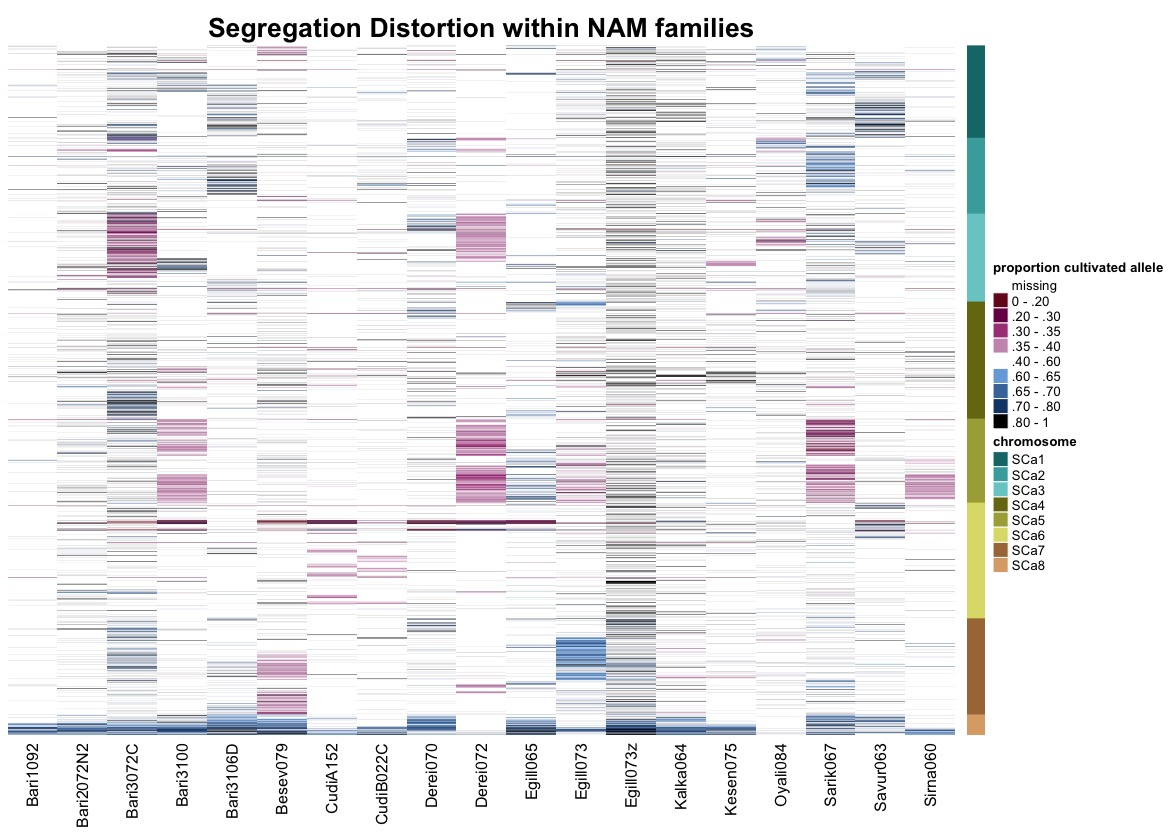
\includegraphics[height = 15cm, width = 15cm]{tex/chickpea/Segdis.jpeg}
    \caption{ Segregation distortion within individual NAM families. Each column represents one NAM family, the wild parent is indicated below the column. Horizontal lines indicate the positions of chromosome boundaries for chromosomes 1 to 10, top to bottom. The proportion of cultivated (ICCV96029) allele for an interval is indicated by the color scale. Chromosome are represented by vertical colour bar.}
    \label{fig:seg-dis}
\end{figure}

\subsection{Phenotypic distributions}
Fig. \ref{fig:pop-dist} seeks to describe family-wise distribution. We see that most of the phenotypes have similar distributions across populations. However, we have some low individuals with low harvest index in the Derei and Sirna families - which concurrently show distortions towards wild allele in fig. \ref{fig:seg-dis}. Low harvest index usually translates to large plants with low fertility and such individuals are good candidates for investigating incompatibility loci. 

Fig. \ref{fig:pheno-corr} looks at phenotypic correlation and distribution of phenotypes across all hybrid families. We can see that most phenotypes are near normally distributed except for shatterring index which we believe to be a more simple trait regulated from a few loci. Perhaps unsurprisingly, many phenotypes show correlation with yield being strongly correlated with `harvest index' and `total plant biomass'. `Plant volume' and `total plant biomass' are similarly correlated. 

\begin{figure}
    \centering
    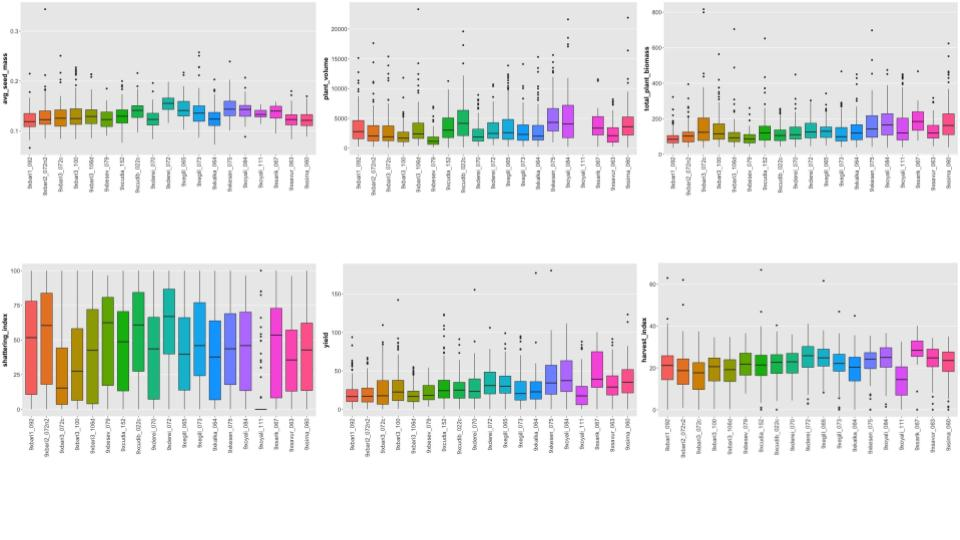
\includegraphics[height = 15cm, width = 15cm]{tex/chickpea/pop-wise-dist.jpg}
    \caption{Population wise distribution of phenotypes. In clockwise order, average seed mass, plant volume, total plant biomass, harvest index, yield and shattering index. X-axis labels indicated the founder that the cultivar was crossed with.}
    \label{fig:pop-dist}
\end{figure}

\begin{figure}
    \centering
    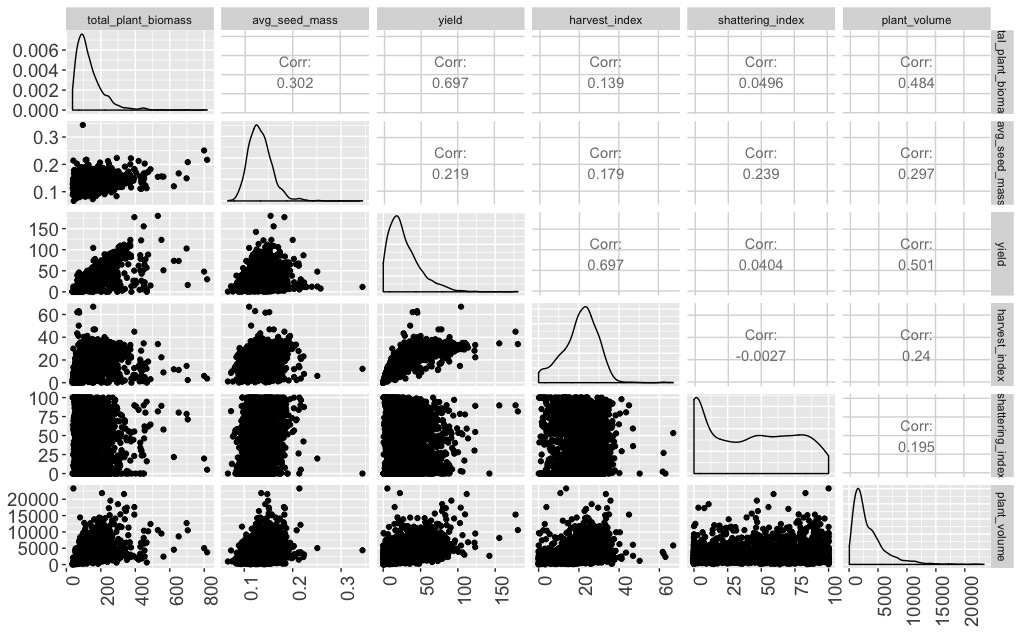
\includegraphics[height = 15cm, width = 15cm]{tex/chickpea/pheno_correlation.jpeg}
    \caption{Phenotypic distribution and correlation across all hybrids. we see that yield is correlated with `harvest index' and `total plant biomass'. Most phenotypes have normal distribution. }
    \label{fig:pheno-corr}
\end{figure}

\subsection{Heritability estimation}

We used GVCBLUP \cite{Wang2014} implementation of the mixed models approach to estimate the additive and dominance contribution to phenotypic variation in the hybrids. As we can see in fig. \ref{fig:varcomp}, the additive contribution is highest for `average seed mass'. This is unsurprising, because most of the selection that has happened in domesticated chickpea is to increase seed size.  A phenotype that has been selected against is shattering, and so perhaps expectedly it too has a strong additive component. We notice that shattering has a very strong dominance component as well, while the other phenotypes show low dominance contributions. 

\begin{figure}
    \centering
    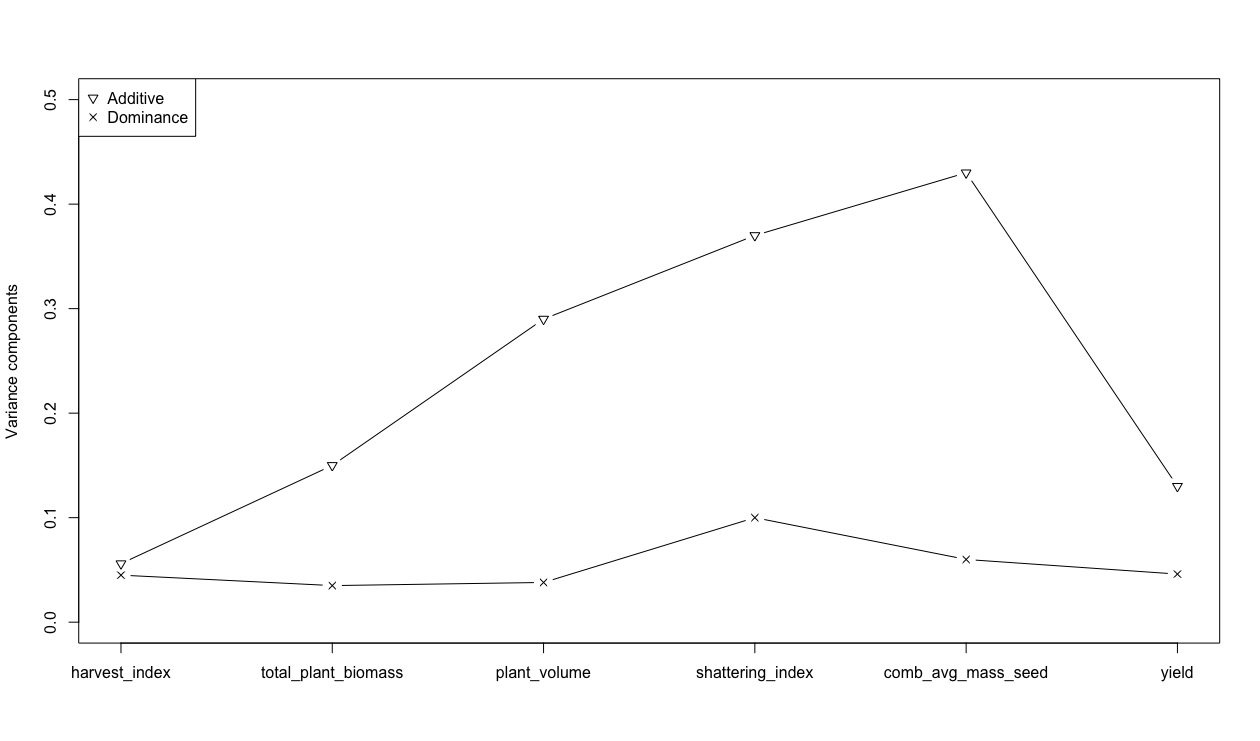
\includegraphics[height = 15cm, width = 15cm]{tex/chickpea/varcomp.jpeg}
    \caption{Additive and dominance variance component estimates of hybrid phenotypes.}
    \label{fig:varcomp}
\end{figure}

\subsection{Single marker analysis}

Finally, we fitted a liner model in which each marker is tested individually for association with the phenotype. As we use a genotypic model, we can tease out additive and dominace deviation effects at each locus. The results for additive effect is presented in fig. \ref{fig:man-add}, for positive dominance in fig. \ref{fig:man-dom} and for over-dominance in fig. \ref{fig:man-over}. 

We see a strong signal for additive effect for shattering on chromosome 6 and chromosome 7. The wild allele in both cases increases the phenotype. Importantly, the wild allele is dominant at chromosome 6 while the locus on chromosome 7 does not seem to have a dominant effect. 

We find significant hits for additive effect for average seed mass, plant volume and plant biomass. However, as expected from the dominance heritability estimates, besides shattering index most phenotypes do not show significance for dominance effect. 

\begin{figure}
    \centering
    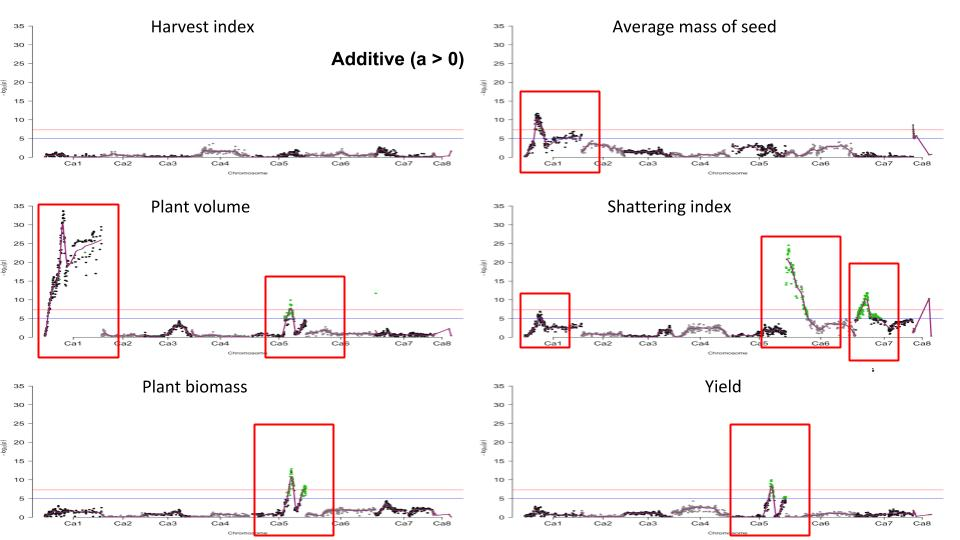
\includegraphics[height=18cm, width=15cm]{tex/chickpea/manhattan-add.jpg}
    \caption{Manhattan plot for p-values of additive effects of all 6 phenotypes. The linear model was set up in such a way that we always interpret the effect of the wild allele in the hybrid. Blue line is for suggestive cut off and red line is for genome wide cut off. In regions that are significant, green dot indicates that the wild allele increases the phenotype.}
    \label{fig:man-add}
\end{figure}

\begin{figure}
    \centering
    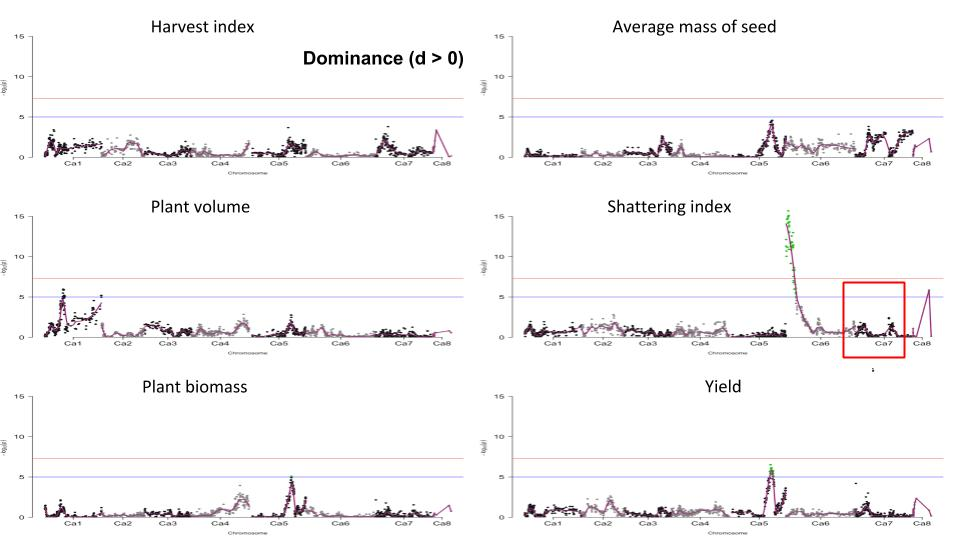
\includegraphics[height=18cm, width=15cm]{tex/chickpea/manhattan-dom.jpg}
    \caption{Manhattan plot for p-values of dominance effects of all 6 phenotypes. The linear model was set up in such a way that we always interpret the effect of the wild allele in the hybrid. Blue line is for suggestive cut off and red line is for genome wide cut off. In regions that are significant, green dot indicates that the wild allele shows dominance and increases the phenotype.}
    \label{fig:man-dom}
\end{figure}

\begin{figure}
    \centering
    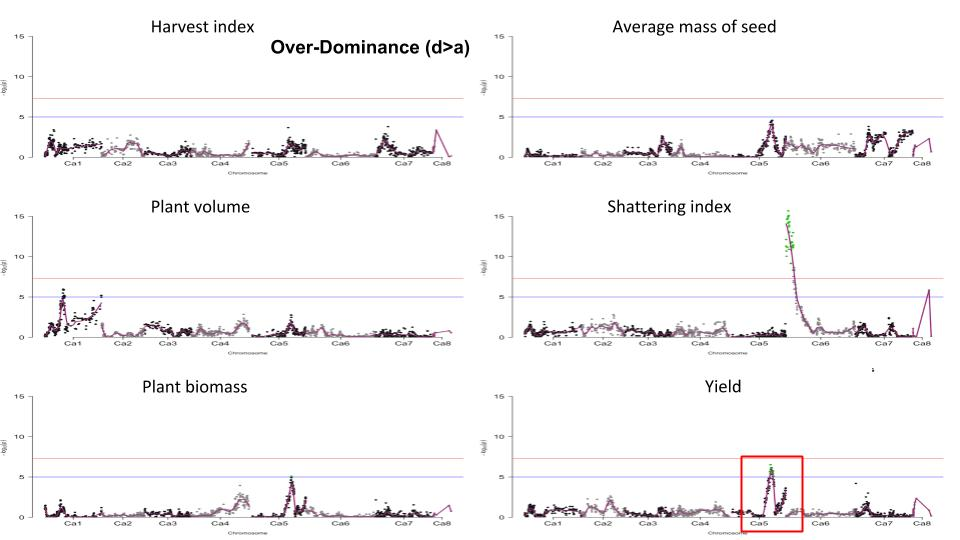
\includegraphics[height=18cm, width=15cm]{tex/chickpea/manhattan-over.jpg}
    \caption{Manhattan plot for p-values of dominance effects of all 6 phenotypes. The linear model was set up in such a way that we always interpret the effect of the wild allele in the hybrid. Blue line is for suggestive cut off and red line is for genome wide cut off. In regions that are significant, green dot indicates that the wild allele shows over-dominance.}
    \label{fig:man-over}
\end{figure}

\section{Conclusion}

Low diversity in domesticated crops is a cause of concern as it reduces resilience of cultivated crops against changes in climatic conditions and ability to resist pathogens. With an increasing population, food security concerns will become more and more acute over the next couple of decades. In such a scenario, it is increasingly imperative to protect existing high yield elite cultivars and produce new breeds that are resilient to changing weather conditions and ecological systems. One possible solution would be to harness diversity back from wild relatives of exiting crop cultivars. 

In order to introgress favourable genomic regions from wilds into elite cultivars, it is necessary to identify the genomic architecture of important agronomic traits. The NAM panels in maize were developed for this explicit purpose and have provided great utility in the breeding program. 

In this chapter, we have introduced the NAM hybrid populations that were grown for chickpea. Since we work with F2 populations, we can also study the dominance architecture of many traits. Here we use GWAS based approaches to study genomic architecture of many traits. We also identify incompatability loci that may point towards viability selection between the two chickpea species. 